% Propósito: mostrar que el máximo de la onda viajera depende de la frecuencia
% y que la extensión espacial también depende del nivel.
% Origen: envolventes analíticas esquemáticas
% y(s)=C(s/s_c)^a exp[a(1-s/s_c)], con 0<=s<=1 y C elegido para fijar
% la escala vertical indicada. En el panel (a),
% a=3 y s_c={0,20; 0,50; 0,80}; cada curva se normaliza a su máximo.
% En el panel (b), s_c=0,55 y se comparan una envolvente estrecha (a=8,
% escala 0,62) y otra más ancha (a=3, escala 1,00). Los parámetros son
% didácticos y no representan datos anatómicos o experimentales.
% Descripción accesible: en el panel superior, tres ondas parten de la base.
% La frecuencia alta alcanza su máximo cerca de la base, la media en la zona
% central y la baja cerca del ápice. En el panel inferior, para una misma
% frecuencia, la señal débil produce una respuesta más estrecha y menor en la
% escala esquemática; la intensa produce una respuesta mayor y más extendida.
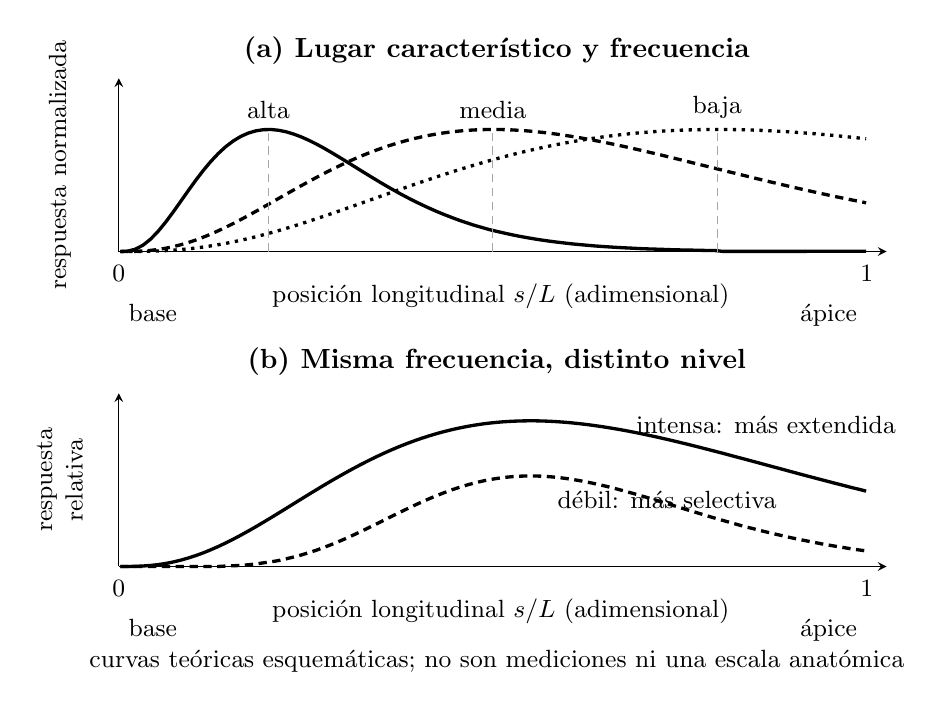
\begin{tikzpicture}[font=\small,>=stealth,x=1cm,y=1cm]
    % Panel (a): tonotopía.
    \node[font=\bfseries] at (5.90,6.20)
        {(a) Lugar característico y frecuencia};
    \draw[->] (1.10,3.65) -- (10.85,3.65);
    \draw[->] (1.10,3.65) -- (1.10,5.85);
    \node[rotate=90] at (0.35,4.75) {respuesta normalizada};
    \node at (5.95,3.08)
        {posición longitudinal \(s/L\) (adimensional)};
    \node[anchor=north] at (1.10,3.60) {\(0\)};
    \node[anchor=north] at (10.60,3.60) {\(1\)};
    \node[anchor=north west] at (1.10,3.10) {base};
    \node[anchor=north east] at (10.60,3.10) {ápice};

    \draw[very thick,samples=100,domain=0.002:1]
        plot ({1.10+9.50*\x},
        {3.65+1.55*pow(\x/0.20,3)*exp(3*(1-\x/0.20))});
    \draw[very thick,densely dashed,samples=100,domain=0.002:1]
        plot ({1.10+9.50*\x},
        {3.65+1.55*pow(\x/0.50,3)*exp(3*(1-\x/0.50))});
    \draw[very thick,dotted,samples=100,domain=0.002:1]
        plot ({1.10+9.50*\x},
        {3.65+1.55*pow(\x/0.80,3)*exp(3*(1-\x/0.80))});

    \draw[densely dashed,black!35] (3.00,3.65) -- (3.00,5.20);
    \draw[densely dashed,black!35] (5.85,3.65) -- (5.85,5.20);
    \draw[densely dashed,black!35] (8.70,3.65) -- (8.70,5.20);
    \node[anchor=south] at (3.00,5.22) {alta};
    \node[anchor=south] at (5.85,5.22) {media};
    \node[anchor=south] at (8.70,5.22) {baja};

    % Panel (b): dependencia del nivel.
    \node[font=\bfseries] at (5.90,2.25)
        {(b) Misma frecuencia, distinto nivel};
    \draw[->] (1.10,-0.35) -- (10.85,-0.35);
    \draw[->] (1.10,-0.35) -- (1.10,1.85);
    \node[rotate=90,align=center] at (0.35,0.75)
        {respuesta\\relativa};
    \node at (5.95,-0.92)
        {posición longitudinal \(s/L\) (adimensional)};
    \node[anchor=north] at (1.10,-0.40) {\(0\)};
    \node[anchor=north] at (10.60,-0.40) {\(1\)};
    \node[anchor=north west] at (1.10,-0.90) {base};
    \node[anchor=north east] at (10.60,-0.90) {ápice};

    \draw[very thick,densely dashed,samples=100,domain=0.002:1]
        plot ({1.10+9.50*\x},
        {-0.35+1.15*pow(\x/0.55,8)*exp(8*(1-\x/0.55))});
    \draw[very thick,samples=100,domain=0.002:1]
        plot ({1.10+9.50*\x},
        {-0.35+1.85*pow(\x/0.55,3)*exp(3*(1-\x/0.55))});
    \node[anchor=west] at (7.55,1.45) {intensa: más extendida};
    \node[anchor=west] at (6.55,0.50) {débil: más selectiva};
    \node[align=center] at (5.90,-1.55)
        {curvas teóricas esquemáticas; no son mediciones ni una escala anatómica};
\end{tikzpicture}
